\documentclass[journal,12pt,twocolumn]{IEEEtran}
%
\usepackage{setspace}
\usepackage{gensymb}
\singlespacing
\usepackage[cmex10]{amsmath}
\usepackage{siunitx}
\usepackage{amsthm}

\usepackage{mathrsfs}

\usepackage{txfonts}
\usepackage{stfloats}

\usepackage{steinmetz}
\usepackage{cite}
\usepackage{cases}
\usepackage{subfig}
\usepackage{longtable}
\usepackage{multirow}
\usepackage{enumitem}
\usepackage{mathtools}
\usepackage{tikz}
\usepackage{circuitikz}
\usepackage{verbatim}
\usepackage{tfrupee}
\usepackage[breaklinks=true]{hyperref}
\usepackage{tkz-euclide} % loads  TikZ and tkz-base
\usetikzlibrary{calc,math}
\usetikzlibrary{fadings}
\usepackage{listings}
    \usepackage{color}                                            %%
    \usepackage{array}                                            %%
    \usepackage{longtable}                                        %%
    \usepackage{calc}                                             %%
    \usepackage{multirow}                                         %%
    \usepackage{hhline}                                           %%
    \usepackage{ifthen}                                           %%
  %optionally (for landscape tables embedded in another document): %%
    \usepackage{lscape}     
\usepackage{multicol}
\usepackage{chngcntr}
\DeclareMathOperator*{\Res}{Res}

\renewcommand\thesection{\arabic{section}}
\renewcommand\thesubsection{\thesection.\arabic{subsection}}
\renewcommand\thesubsubsection{\thesubsection.\arabic{subsubsection}}

\renewcommand\thesectiondis{\arabic{section}}
\renewcommand\thesubsectiondis{\thesectiondis.\arabic{subsection}}
\renewcommand\thesubsubsectiondis{\thesubsectiondis.\arabic{subsubsection}}

\hyphenation{op-tical net-works semi-conduc-tor}
\def\inputGnumericTable{}                                 %%

\lstset{
%language=C,
frame=single, 
breaklines=true,
columns=fullflexible
}
\begin{document}
%


\newtheorem{theorem}{Theorem}[section]
\newtheorem{problem}{Problem}
\newtheorem{proposition}{Proposition}[section]
\newtheorem{lemma}{Lemma}[section]
\newtheorem{corollary}[theorem]{Corollary}
\newtheorem{example}{Example}[section]
\newtheorem{definition}[problem]{Definition}
\newcommand{\BEQA}{\begin{eqnarray}}
\newcommand{\EEQA}{\end{eqnarray}}
\newcommand{\define}{\stackrel{\triangle}{=}}
\bibliographystyle{IEEEtran}
\providecommand{\mbf}{\mathbf}
\providecommand{\pr}[1]{\ensuremath{\Pr\left(#1\right)}}
\providecommand{\qfunc}[1]{\ensuremath{Q\left(#1\right)}}
\providecommand{\sbrak}[1]{\ensuremath{{}\left[#1\right]}}
\providecommand{\lsbrak}[1]{\ensuremath{{}\left[#1\right.}}
\providecommand{\rsbrak}[1]{\ensuremath{{}\left.#1\right]}}
\providecommand{\brak}[1]{\ensuremath{\left(#1\right)}}
\providecommand{\lbrak}[1]{\ensuremath{\left(#1\right.}}
\providecommand{\rbrak}[1]{\ensuremath{\left.#1\right)}}
\providecommand{\cbrak}[1]{\ensuremath{\left\{#1\right\}}}
\providecommand{\lcbrak}[1]{\ensuremath{\left\{#1\right.}}
\providecommand{\rcbrak}[1]{\ensuremath{\left.#1\right\}}}
\theoremstyle{remark}
\newtheorem{rem}{Remark}
\newcommand{\sgn}{\mathop{\mathrm{sgn}}}
\providecommand{\abs}[1]{\left\vert#1\right\vert}
\providecommand{\abs}[1]{\lvert#1\rvert} 
\providecommand{\res}[1]{\Res\displaylimits_{#1}} 
\providecommand{\norm}[1]{\left\lVert#1\right\rVert}
%\providecommand{\norm}[1]{\lVert#1\rVert}
\providecommand{\mtx}[1]{\mathbf{#1}}
\providecommand{\mean}[1]{E\left[ #1 \right]}
\providecommand{\fourier}{\overset{\mathcal{F}}{ \rightleftharpoons}}
%\providecommand{\hilbert}{\overset{\mathcal{H}}{ \rightleftharpoons}}
\providecommand{\system}{\overset{\mathcal{H}}{ \longleftrightarrow}}
	%\newcommand{\solution}[2]{\textbf{Solution:}{#1}}
\newcommand{\solution}{\noindent \textbf{Solution: }}
\newcommand{\cosec}{\,\text{cosec}\,}
\providecommand{\dec}[2]{\ensuremath{\overset{#1}{\underset{#2}{\gtrless}}}}
\newcommand{\myvec}[1]{\ensuremath{\begin{pmatrix}#1\end{pmatrix}}}
\newcommand{\mydet}[1]{\ensuremath{\begin{vmatrix}#1\end{vmatrix}}}
\numberwithin{equation}{subsection}
\makeatletter
\@addtoreset{figure}{problem}
\makeatother
\let\StandardTheFigure\thefigure
\let\vec\mathbf
\renewcommand{\thefigure}{\theproblem}
\def\putbox#1#2#3{\makebox[0in][l]{\makebox[#1][l]{}\raisebox{\baselineskip}[0in][0in]{\raisebox{#2}[0in][0in]{#3}}}}
     \def\rightbox#1{\makebox[0in][r]{#1}}
     \def\centbox#1{\makebox[0in]{#1}}
     \def\topbox#1{\raisebox{-\baselineskip}[0in][0in]{#1}}
     \def\midbox#1{\raisebox{-0.5\baselineskip}[0in][0in]{#1}}
\vspace{3cm}
\title{ASSIGNMENT-16}
\author{R.YAMINI}
\maketitle
\newpage
\bigskip
\renewcommand{\thefigure}{\theenumi}
\renewcommand{\thetable}{\theenumi}


%
\section{QUESTION No-8.6 (GATE Probability)}
Suppose $X$ and $Y$ are two random variables such that $aX + bY$ is a normal random variable for all $a,b \in \mathbb{R}$. Consider the following statements P,Q,R and S: \\
(P): $X$ is a standard normal random variable.\\
(Q): The conditional distribution of $X$ given $Y$ is normal.\\
(R): The conditional distribution of $X$ given $X$ + $Y$ is normal.\\
(S): $X$ - $Y$ has mean $0$.\\
 Which of the above statements ALWAYS hold TRUE?
\begin{enumerate}
\begin{multicols}{2}
\setlength\itemsep{2em}

\item both P and Q
\item both Q and R
\item both Q and S
\item both P and S

\end{multicols}
\end{enumerate}
\section{Solution}
\begin{definition}
Two random variables $X$ and $Y$ are said to be bivariate normal, or jointly normal, if $aX+bY$ has a normal distribution for all $a,b \in \mathbb{R}$.
\end{definition}
(P) $X$ is a standard normal random  variable.\\
Let,
\begin{align}
 a=1,b=0  \\
  \implies X \text{is normal}.
\end{align}
 Similarly let
 \begin{align}
    a=0,b=1 \\
    \implies Y \text{is normal}.
 \end{align}
The given information is not sufficient to conclude whether $X$ is a standard normal random variable.
Thus this statement does not hold true always.
\\
(Q) The conditional distribution of $X$ given $Y$ is normal.\\
\begin{theorem}
Let $X$ and $Y$ be two bivariate normal random variables then there exist independent standard normal random variables $Z_1$ and $Z_2$ such that \label{T1}
\begin{align}
    X&=\sigma_X (\rho Z_1 +\sqrt{1-\rho^2} Z_2)+\mu_X  \\
    Y&=\sigma_Y Z_1+\mu_Y 
 \end{align}
\end{theorem}
By using theorem \ref{T1} we show that the statement Q is true.Thus given $Y=y$, we have
\begin{align}
Z_1=\frac{y-\mu_Y}{\sigma_Y},\\
\implies X&=\sigma_X (\rho\frac{y-\mu_Y}{\sigma_Y} +\sqrt{1-\rho^2} Z_2)+\mu_X .
\end{align}
Since $Z_1$ and $Z_2$ are independent we have,
\begin{equation}
    \begin{aligned}
  E[X|Y=y]&= \sigma_X \brak{\rho\frac{y-\mu_Y}{\sigma_Y}} \\ &+\sigma_X\brak{\sqrt{1-\rho^2} E[Z_2]}+\mu_X
  \end{aligned}
\end{equation}
\begin{align}
 &=\mu_X+ \rho \sigma_X \frac{y-\mu_Y}{\sigma_Y},\\
  Var(X|Y=y)&=(1-\rho^2)\sigma^2_X.     
\end{align}
where $\mu_X$ and $\sigma_X$ denote the mean and standard deviation of random variable $X$ similarly $\mu_Y$ and $\sigma_Y$ denote the mean and standard deviation of random variable $Y$ and thus 
\begin{align}
   X|Y \sim N\brak{\mu_X+\rho\frac{\sigma_X}{\sigma_Y}\brak{Y-\mu_X},\sigma_X\brak{\sqrt{1-\rho^2}}} 
\end{align}
 Thus the statement holds true always.
 The result is verified using python below
 \numberwithin{figure}{section}
\begin{figure}[!ht]
\centering
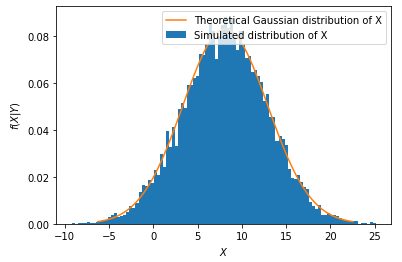
\includegraphics[width=\columnwidth]{X given Y.PNG}
\caption{Graphical representation(Q) - X given Y is normal.}
\label{fig:Graphical Solution}	
\end{figure}
\\
(R) The conditional distribution of $X$ given $X$ + $Y$ is normal.\\
Let,
\begin{align}
a=1, b=1 \\
\implies X+Y \text{is normal}
\end{align}
and let $Z=X+Y$ then $f_{X|Z}$ is also normal which follows from the previous statement.
Thus the statement holds true always.
The result is verified using python below
 \numberwithin{figure}{section}
\begin{figure}[!ht]
\centering
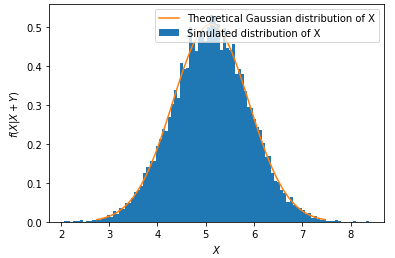
\includegraphics[width=\columnwidth]{X given X+Y.PNG}
\caption{Graphical representation(R) - X given X+Y is normal.}
\label{fig:Graphical Solution}	
\end{figure}
\\
(S) $X$ - $Y$ has mean $0$.\\
In general
\begin{align}
    E[aX+bY] &= aE[X]+bE[Y] \\
    Var(aX+bY) &= a^2Var(X)+2abCov(X,Y)+b^2Var(Y)
\end{align}
For $a=1$ and $b=-1$ we have
\begin{align}
  E[X-Y] &= E[X]-E[Y] \\
    Var(X-Y) &= Var(X)-2Cov(X,Y)+Var(Y)  
\end{align}
Mean of $X-Y$ is 0 only when $X$ and $Y$ are independent standard normal variable and the given information is not sufficient to conclude. Thus this statement does not hold true always. 
\end{document}
